\chapter{Úvod}
Tématem této diplomové práce jsou metody automatizace testů síťových prvků. Nejdříve bychom měl popsat definici testování a různé způsoby jak je možné testování provádět. Definice testování je podle IEEE Software Engineering Body of Knowledge (SWEBOK 2004) následující:

"Softwarové testování se skládá z dynamického ověřování chování programu proti očekávanému chování programu na konečné množině testovacích případů vhodně vybraných z obvykle nekonečné množiny případů."

Na způsoby testování lze pohlížet několika pohledy. Prvním pohledem na testování je rozdělení na šest jednotlivých úrovní testování. Mezi tyto úrovně testování patří testování programátorem, testování jednotlivých jednotek kódu, funkční testování, integrační testování, systémové testování a akceptační testy. Všechny úrovně budou detailně popsány v kapitole používané metody testování. Dalším pohledem na kategorizaci testování je způsob provádění testů. Prvním způsobem je manuální testování, kdy tester manuálně provádí testy podle předem daných testovacích procedur. Dokonalejším způsobem testování je takzvané automatizované testování, kdy testy jsou prováděny automaticky dle předem napsaných testovacích procedur. Testovací procedury jsou psány testery či vývojáři. Všechny testovací procedury musí být přepisovány při změně funkcionality výrobku, nebo při přidání nového výrobku. Tímto přístupem je ušetřeno spoustu času, který byl plýtván opakovaným manuálním testováním identických věcí. Posledním známým a v dnešní době moderním způsobem testování je testování založené na modelech. U tohoto způsobu testování je vytvořen model testované oblasti, či zařízení a automaticky se generují testovací procedury. Způsob testování založeného na modelech ušetří další čas trávený úpravami a tvorbou dalších testovacích procedur při změně funkcionality softwaru či přidání nového produktu, jelikož je upravován pouze model zařízení. Testovací systém, který bude výstupem této diplomové práce, by měl testovat zařízení na úrovni systémového testování. Systémové testy by měl testovací systém pro konkrétní zařízení vybírat a  provádět automatizovaně pomocí testování založeného na modelech.

\section{Praktické využití}
Praktická implementace testovacího systému bude provedena pro testování výrobků společnosti Conel, ze které přišel požadavek na toto zadání. Zadání diplomové práce jsem si vybral, jelikož ve společností pracuji na různých pozicích již 4 roky. Způsoby testování výrobku se během fungování firmy měnily následujícím způsobem. Zpočátku, kdy počet modelů routerů byl velmi malý a routery vyvíjel pouze jeden programátor bylo prováděno pouze testování programátorem a následovali až akceptační testy u zákazníka. Při rostoucím počtu modelů, funkcionalit a počtu vývojářů byl tento systém již dále neudržitelný a mezi testy programátorem a akceptačními testy musely být vloženy systémové testy prováděny testerem podle testovacích procedur. Dnes, kdy počet modelů routerů přesahuje 30 základních modelů a nové funkcionality  přibývají čím dál tím rychleji, je tento systém taktéž dále neudržitelný. Již nyní by kompletní testování všech funkcionalit na všech typech routerů trvalo přibližně měsíc práce v jednom člověku.

\begin{figure}[h]
	\centering
	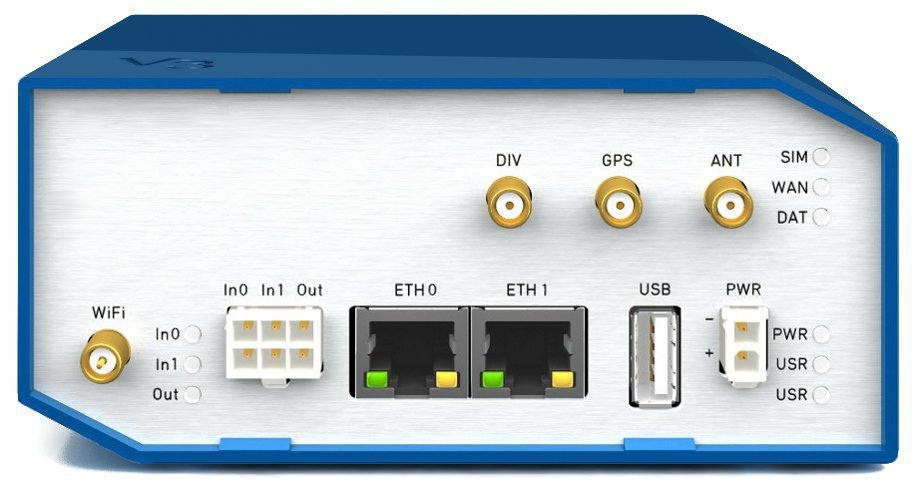
\includegraphics[width=.6\LW]{router}
	\caption{Příklad routeru}
	\label{fig:router}
\end{figure}

Na základě těchto skutečností byl vznešen požadavek na testovací systém, pomocí kterého bude možné automaticky testovat aktuálně vyvíjený firmware na všech vyráběných modelech routerů a jejich volitelných portech. Zvolena byla kombinace integračního testování a testování založené na modelech. Testování bude pokrývat pouze integrační a systémové testování, jelikož z větší části je firmware testovaných výrobků tvořen opensource programy. Psaní unit testů pro každý open source program je časově a složitostně nepřínosné. Systémové testování by mělo probíhat alespoň jednou denně, aby bylo možno případné chyby odchytnout již během vývoje firmwaru a tím usnadnilo a zrychlilo vývoj samotný. Dalším velikým přínosem je zkvalitnění samotného testování, jelikož testovací technici mohou vymýšlet nové testovací procedury a situace, namísto opakovaného manuálního testování stejných procedur.

\section{Aktuálnost}
Testování každého výrobku před uvedením na trh, či testováním nového firmwaru před jeho vydáním je velmi důležitá součást vývoje a neměla by se opomíjet. Hlavním důvodem průběžného testování kompletní funkcionality zařízení je dobré jméno u zákazníka, který nemá zájem o výrobek plný chyb. Dalším důvodem průběžného testování je méně práce pří pozdějším opravování způsobených chyb. Při zvyšování počtu výrobků a funkcionalit je nutné zvyšovat počet testovacích pracovníků, nebo změnit přístup k způsobu testování. Jelikož první řešení se zdá být na první pohled neefektivní, tak se v této práci vydám druhou cestou. Při zvyšování efektivity testů použiju automatizované testování. Dále pokud to bude možné a alespoň trochu efektivní využiji dnes velmi moderní metodu testování založeného na modelech. Každému zařízení by měl být vytvořen model, pomocí kterého budou na určených zařízeních spouštěny vybrané testy s danými parametry. V dnešní době byrokracie tento systém také pomůže ke shromažďování všech testovacích procedur a reportů ze všech provedených testů na jednom místě.

\section{Výstup práce}
Hlavním cílem práce je hotové řešení automatizovaného systémového řešení testování všech modelů bezdrátových routerů společnosti Conel. Výstupem  řešení bude testovací laboratoř obsahující všechny výrobky, pomocné síťové prvky a testovací server. Dalším výstupem bude aplikace na obstarávající režii a spouštění testů, interface pro zobrazování reportů ze všech testů s možností administrace testovacího systému. Poslední cíl je vytvoření testovacích procedur pro testování jednotlivých funkcí bezdrátových routerů společnosti Conel.

\section{Struktura práce}
Celou diplomovou práci lze rozdělit do třech hlavních částí. V první teoretické částí budou rozebírány všechny různé metody a přístupy k testování samotnému, aby bylo možné dále stavět na teoretickém základu. Dále v teoretické části budou prozkoumány všechny možné dostupné produkty určené k samotnému testování, či produkty sloužící k jednotlivým úkonům potřebným pro testování daných produktů. Zde bude kladena snaha využít co nejvíce kvalitních hotových řešení sloužících k účelům testování výrobků společnosti Conel. Ideální cesta by byla nalézt produkt sloužící k našemu účelu, ale jelikož je požadavek velmi specifický, s velkou pravděpodobností bude potřeba z velké části testovací systém vyvinout. Druhá část práce se bude zabývat praktickým návrhem všech částí zabývající se testováním každého routeru. V první fázi bude navrhnuta testovací laboratoř z hlediska potřebného hardwaru. Dále bude popsán návrh a implementace programu zajišťující samotné testování a úkony s testováním související. Následuje kapitola věnující se uživatelskému interfacu pro reportování výsledků a administraci samotného testování. Samostatná kapitola popisuje API pro snadné dopisování nových testovacích procedur. Základní API bude dodáno s testovacím programem a dále bude popsána možnost dopisování nových specifických programů. Stěžejní části je kapitola popisující testovací procedury jednotlivých funkcionalit. Poslední částí je praktická implementace testovací laboratoře a testování celého systému. Výstupy z tohoto testování budou použity v poslední kapitole zabývající se možností budoucího vylepšení a rozšíření testovacího systému.

\endinput
